\section{Convertitore RMS}
Si è realizzato il convertitore RMS in \fig{RMS}, facendo uso dell'integrato AD736.

	\begin{figure}[H]
		\begin{minipage}{0.70\textwidth}
			\centering
			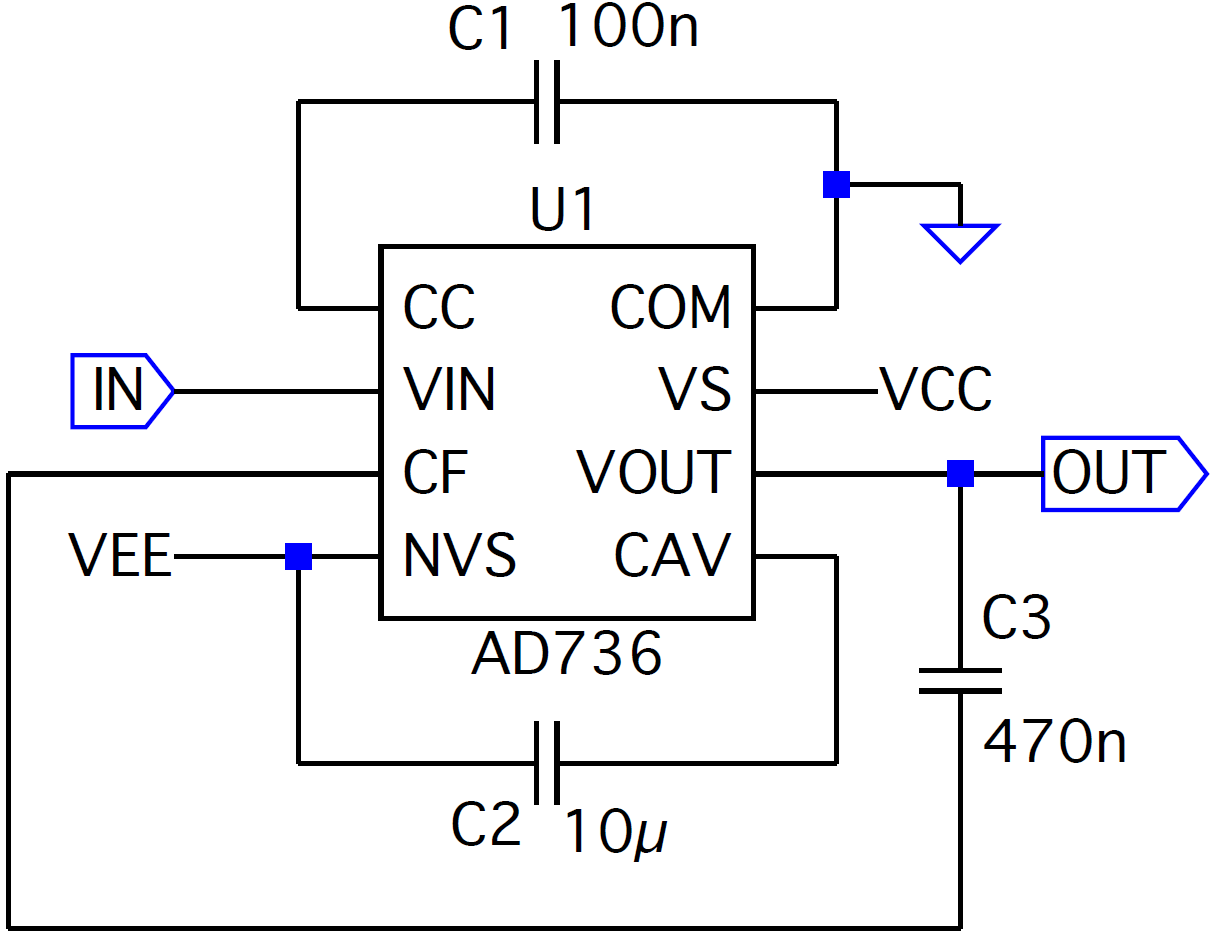
\includegraphics[width=0.5\textwidth]{RMS.png}
			\caption{Circuito del convertitore RMS.}
			\label{fig:RMS}
		\end{minipage}
		\begin{minipage}{0.29\textwidth}
			\begin{tabular}{l@{ }c@{ }l}
				$C_{1}$& = &\SI{114(5)}{\nano\farad}\\
				$C_{2}$& = &\SI{10.3(4)}{\micro\farad}\\
				$C_3$& = &\SI{474(19)}{\nano\farad}\\
			\end{tabular}
		\end{minipage}
	\end{figure}

Si è quindi verificato (vedi \fig{RMS_test}) che il circuito si comportasse come atteso, ovvero che producesse a partire da un segnale AC con ampiezza picco-picco $V_{pp}$ in ingresso, un segnale DC di ampiezza $\frac{V_{pp}}{2\cdot \sqrt{2}}$.

	\begin{figure}[H]
		\centering
		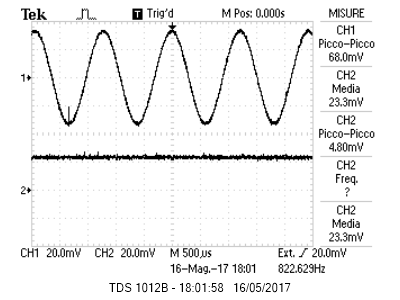
\includegraphics[scale = 0.7]{RMSficator.png}
		\caption{Verifica di funzionamento del RMS converter}
		\label{fig:RMS_test}
	\end{figure}

Il rapporto tra i segnali misurato è di $0.343 \pm 0.008$ a fronte di un valore atteso di $\frac{1}{2\cdot\sqrt{2}} \simeq 0.353$, compatibili quindi entro poco più di $1\sigma$.

\section{Misure di rumore}
Si è quindi proceduto alla misura del rumore al variare della resistenza. Il range di resistenze utilizzate varia tra $\SI{1}{\kilo\ohm}$, appena sufficiente a distinguere una differenza rispetto alla resistenza nulla, e $\SI{100}{\kilo\ohm}$, valore oltre il quale il circuito raggiunge il valore di saturazione (l'OpAmp del post-amplificatore risulta infatti saturato)\footnote{Al variare delle resistenze il valore di saturazione in output viene raggiunto molto prima di quanto atteso e in maniera discontinua rispetto alla legge di andamento attesa. Si sospetta che l'effetto sia dovuto ad effetti di induzione sulla resistenza.}.

I dati raccolti sono riportati in \tab{data} in Appendice. Poiché nella lettura dei valori di tensione l'ultima cifra non era stabile, si è proceduto a stimare l'errore osservando l'intervallo di variabilità delle letture.

Si è proceduto a fittare le misure eseguite con una legge del tipo
$$V_{RMS} = V_{0n} \cdot \sqrt{1+\frac{R}{R_T} + \frac{R^2}{R_n^2}}$$
dove $R$ è la resistenza in ingresso, $V_{0n}$ è il rumore in uscita a resistenza nulla, $R_T$ è la resistenza equivalente del rumore serie dell’amplificatore riferito all’ingresso e $R_n$ è il rapporto tra il rumore parallelo ed il rumore serie dell’amplificatore,
riferiti all’ingresso.

I risultati del fit sono stati:
$$V_{0n} = \SI{61(3)}{\milli\volt} \qquad R_T = \SI{7.3(19)}{\kilo\ohm} \qquad R_n = \SI{19.7(22)}{\kilo\ohm}$$
$$ \text{corr}(V_{0n},R_T)=0.88 \qquad \text{corr}(V_{0n},R_n)=-0.17 \qquad \text{corr}(R_T,R_n)=-0.53$$

Con un $\chi^2 / \text{ndof} = 15.9 / 10$ e un $p = 10.4 \%$.

Il grafico dei dati e del fit è riportato in \fig{fit_rumore}.

	\begin{figure}[H]
		\centering
		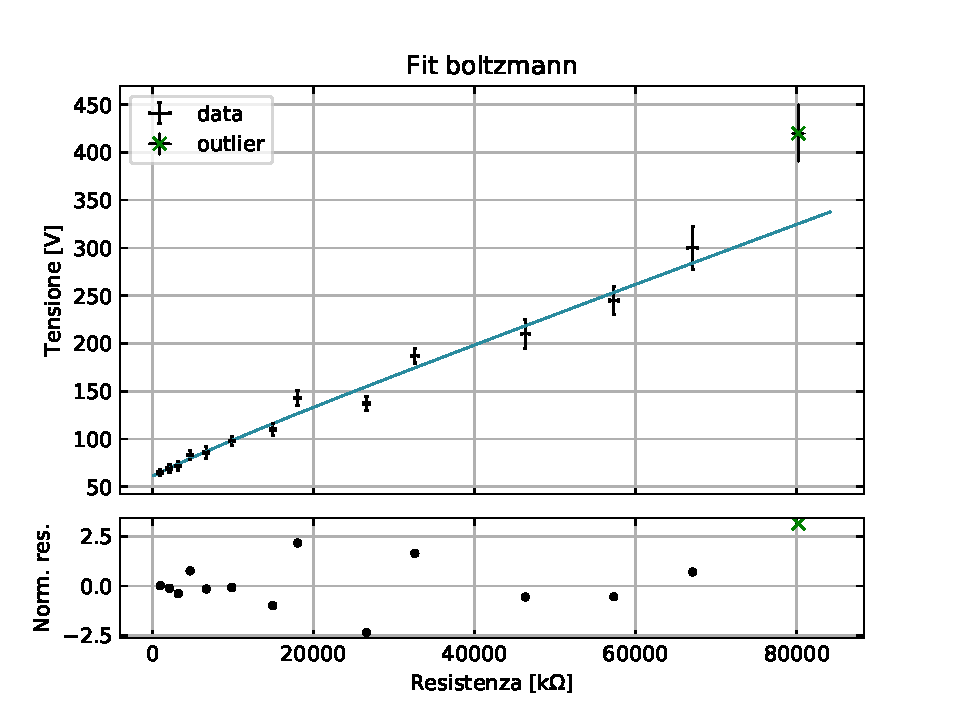
\includegraphics[scale = 1]{fit_dati_rummore.pdf}
		\caption{Grafico dei dati e del fit delle misure di rumore}
		\label{fig:fit_rumore}
	\end{figure}

A partire dalle relazioni che legano i parametri fittati alla costante di Boltzamnn è possibile ricavarne una stima:
$$ k_B = \frac{V_{0n}}{4R_T T A_0^2 \Delta f}$$
\begin{itemize}
	\item $V_{0n}$ e $R_T$ sono i parametri fittati precedentemente (nel propagare l'errore si è tenuto conto della forte correlazione);
	\item $T$ è la temperatura in Kelvin della resistenza, che si è stimata in $\SI{300(3)}{\K}$;
	\item $A_0$ è l'amplificazione totale del circuito, che in virtù delle misure precedenti è $\SI{214(8)e3}{}$;
	\item $\Delta f$ è larghezza di banda del filtro passa banda: $\SI{708(26)}{\hertz}$.
\end{itemize}

Si ottiene quindi $k_B = \SI{1.31(23)e-23}{\J \per \kelvin^{-1}}$, perfettamente compatibile con il valore noto di $\SI{1.38e-23}{\J \per \kelvin^{-1}}$.
